\documentclass[a4paper]{jsarticle}
\usepackage[dvipdfmx]{graphicx}
\usepackage{amsmath}
\renewcommand{\thesection}{第\arabic{section}問}
\renewcommand{\thesubsection}{(\arabic{subsection})}
\renewcommand{\thesubsubsection}{(\alph{subsubsection})}
\begin{document}

\title{2020 分野1}
\author{nakao}
\maketitle

\section{}
\subsection{}
部材の軸に垂直な断面は変形後も軸に垂直であること。

\subsection{}
\begin{figure}[htb]
  \centering
  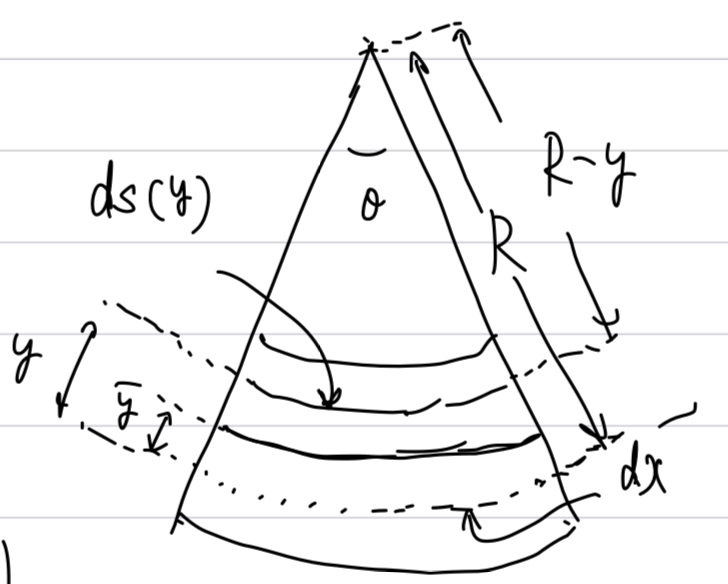
\includegraphics[width=0.3\hsize]{fig1.png}
  \caption{部材微小部分の変形形状}
\end{figure}
変形後の部材形状を扇形と見たときの中心角を$\theta$、変形後の軸方向の長さを$y$の関数として$ds(y)$とする。中立軸ではひずみが0であるから、$ds(0)=dx$であり、
\begin{equation}
  \begin{aligned}
    R \theta &= dx \\
    (R - y) \theta &= ds(y)
  \end{aligned}
\end{equation}
が成り立つ。軸ひずみ$\varepsilon_{xx}$は、
\begin{equation}
  \varepsilon_{xx} = \frac{ds(y) - dx}{dx} = -\frac{y \theta}{R \theta} = -\frac{y}{R}
\end{equation}
となる。

\subsection{}
応力$\sigma_{xx}$は、
\begin{equation}
  \sigma_{xx} = 
  \begin{cases}
    E_1 \varepsilon_{xx} & (\bar{y} \leq y \leq y + h) \\
    E_2 \varepsilon_{xx} & (\bar{y} - h \leq y \leq \bar{y})
  \end{cases} \\
  = 
  \begin{cases}
    -\frac{E_1 y}{R} & (\bar{y} \leq y \leq y + h) \\
    -\frac{E_2 y}{R} & (\bar{y} - h \leq y \leq \bar{y})
  \end{cases}
\end{equation}
であるから、応力分布は下の図のようになる。
\begin{figure}[hbt]
  \centering
  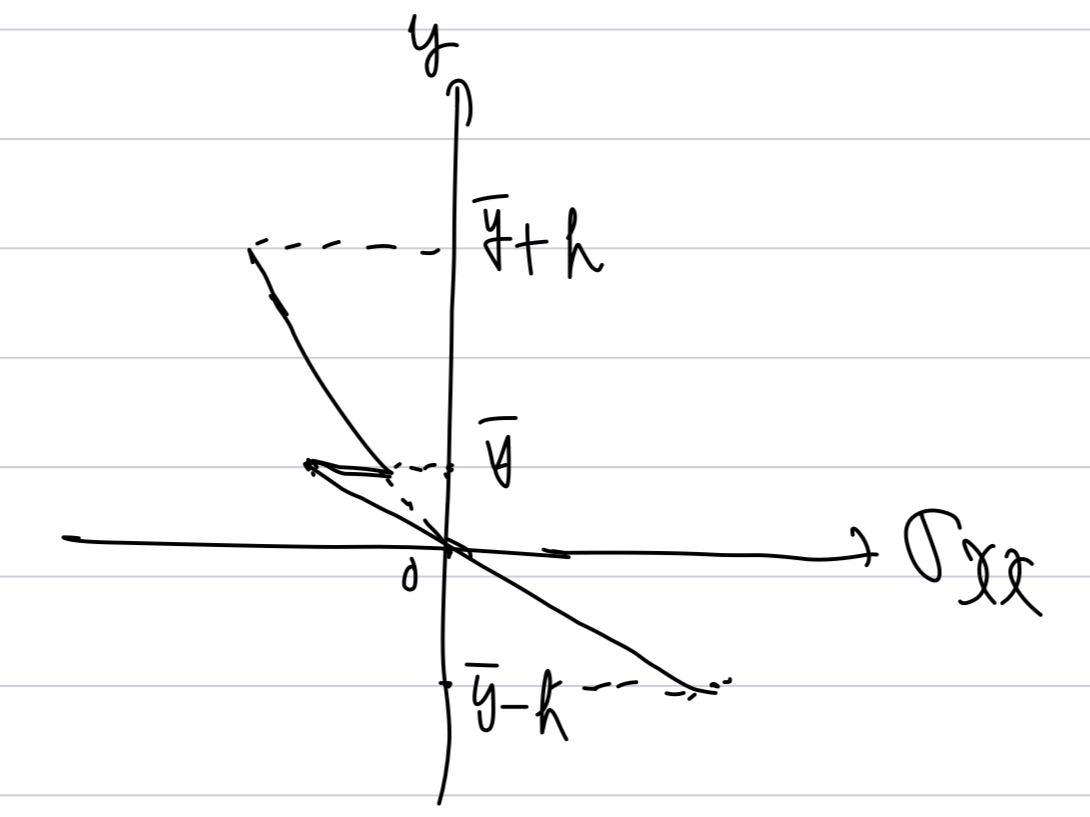
\includegraphics[width=0.5\hsize]{fig2.png}
  \caption{応力分布}
\end{figure}

\subsection{}
満たすべき条件は、
\begin{equation}
  \iint \sigma_{xx} \mathrm{d} A = 0 
\end{equation}
である。
\begin{equation}
  \begin{aligned}
    \iint \sigma_{xx} \mathrm{d} A &= 
    \int_{\bar{y} - h}^{\bar{y} + h} \sigma_{xx} w \mathrm{d} y \\
    &= \int_{\bar{y} - h}^{\bar{y}} \left(-\frac{E_2}{R} y \right) w \mathrm{d} y
    + \int_{\bar{y}}^{\bar{y} + h} \left(-\frac{E_1}{R} y \right) w \mathrm{d} y \\
    &= -\frac{E_1 + E_2}{R} w \bar{y} h + \frac{E_2 - E_1}{2 R} w h^2
  \end{aligned}
\end{equation}
であり、これが0になるためには、
\begin{equation}
  \bar{y} = \frac{E_2 - E_1}{2 (E_1 + E_2)} h
\end{equation}

\subsection{}
モーメントのつり合いから
\begin{equation}
  M = \iint \sigma_{xx} y \mathrm{d} A
\end{equation}
である。これを計算すると、
\begin{equation}
  \begin{aligned}
    M &= \iint \sigma_{xx} y \mathrm{d} A \\
    &= \int_{\bar{y} - h}^{\bar{y} + h} \sigma_{xx} y w \mathrm{d} y \\
    &= \int_{\bar{y} - h}^{\bar{y}} \left(-\frac{E_2}{R} y^2\right) w \mathrm{d} y
    + \int_{\bar{y}}^{\bar{y} + h} \left(-\frac{E_1}{R} y^2\right) w \mathrm{d} y \\
    &= - \frac{2 E_1}{3 R} w h (6 \bar{y}^2 - 3 \bar{y} h + 2 h^2)
  \end{aligned}
\end{equation}
となる。

\subsection{}
クラック発生直後から2本の梁が独立に曲げを受けると考えると、応力分布は下の図のようになる。
\begin{figure}[htb]
  \centering
  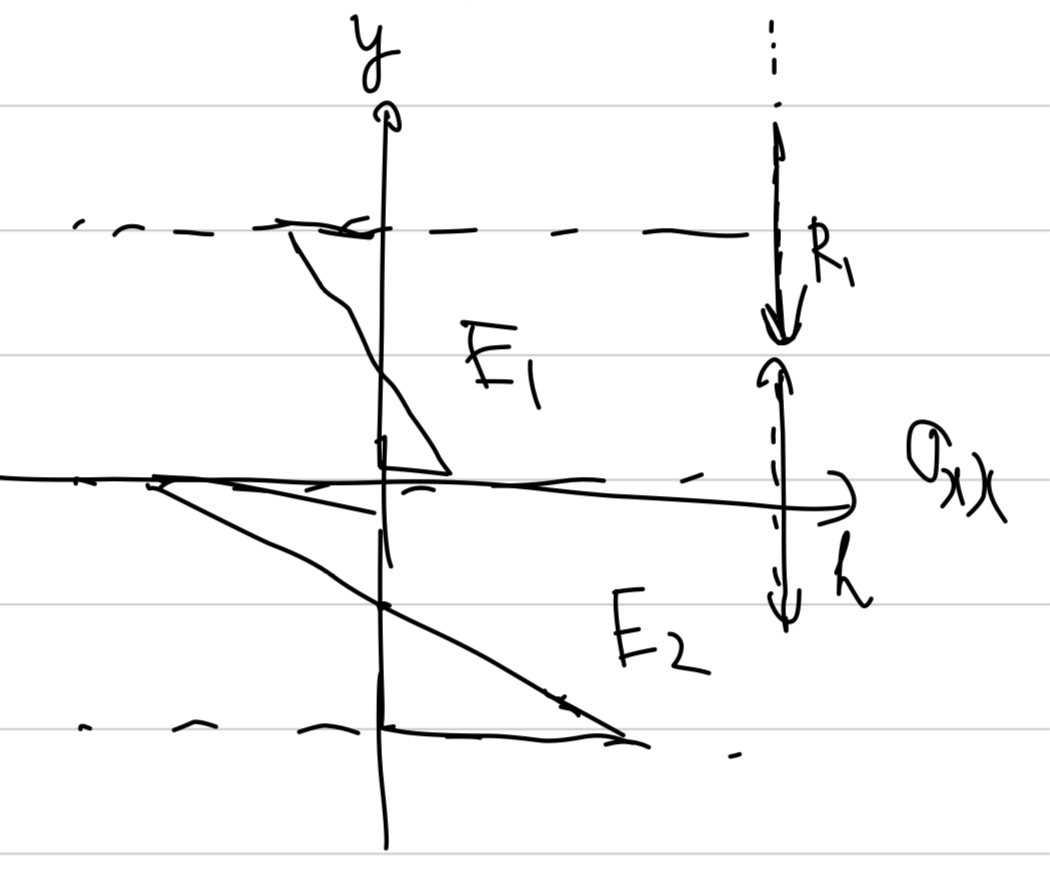
\includegraphics[width=0.3\hsize]{fig3.png}
  \caption{クラック発生後の応力分布}
\end{figure}
上側の梁で変形時の中立軸の曲率半径を$R_1$とすると、モーメントのつりあいから、
\begin{equation}
  \begin{aligned}
    M &= \iint \sigma_{xx} y \mathrm{d} A \\
    &= \int_{-h/2}^{h/2} E_1 \left(-\frac{y}{R_1}\right) w \mathrm{d} y
    + \int_{-h/2}^{h/2} E_2 \left(-\frac{y}{R_1 + h}\right) w \mathrm{d} y \\
    &= \int_{-h/2}^{h/2} E_1 \left(-\frac{y}{R_1}\right) w \mathrm{d} y
    + \int_{-h/2}^{h/2} 3 E_1 \left(-\frac{y}{R_1 + h}\right) w \mathrm{d} y \\
    &= -\frac{4 R_1 + h}{12 R_1 (R_1 + h)} E_1 w h^3
  \end{aligned}
\end{equation}
である。$h$が$R_1$に比べて十分小さいとすると、$4 R_1 + h \simeq 4 R_1, R_1 + h \simeq R_1$より、
\begin{equation}
  M = -\frac{E_1 w h^3}{3 R_1}
\end{equation}
と表せる。一方、$E_2 = 3 E_1$と式(6)より$\bar{y} = h/4$であり、これを用いて式(8)は、
\begin{equation}
  M = -\frac{13 E_1 w h^2}{12 R}
\end{equation}
と表せる。クラック発生前後でモーメントが同一であるとすると、式(10),(11)より
\begin{equation}
  R_1 = \frac{4}{13} R
\end{equation}
を得る。よって、クラック発生前の中立軸における曲率半径は$R$から$R_1 + h/2 + \bar{y} \simeq 4 R /13$に変化する。曲率半径が小さくなっているから変形は大きくなっている。

\section{}
\begin{figure}[htb]
  \centering
  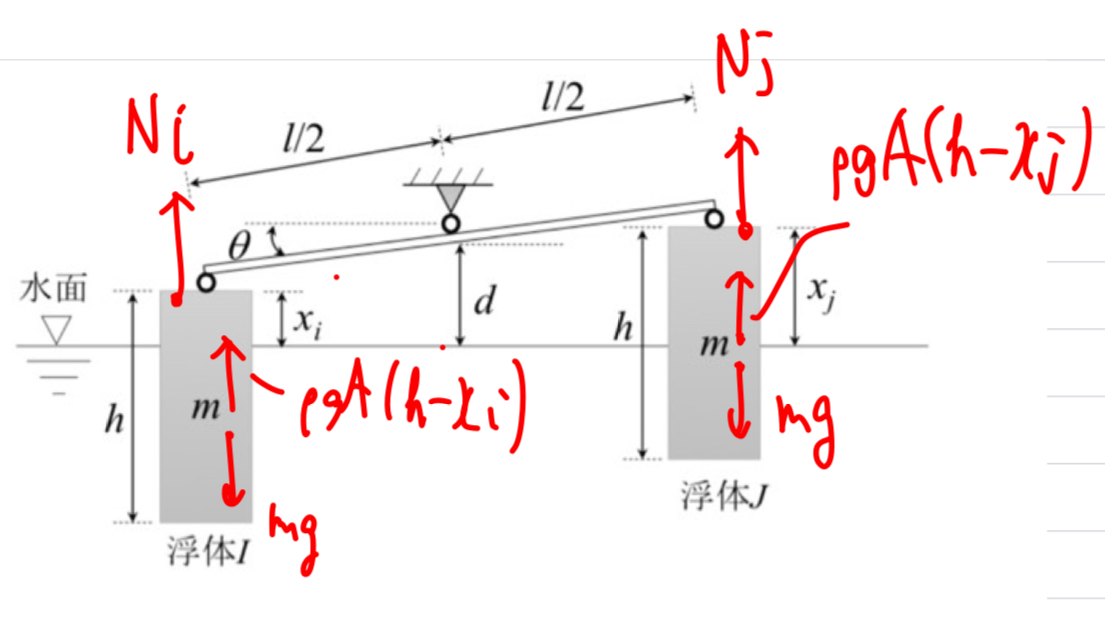
\includegraphics[width=0.6\hsize]{fig4.png}
  \caption{問題設定}
\end{figure}

\subsection{}
\subsubsection{}
浮体$I,J$が連結棒から受ける力をそれぞれ$N_i, N_j$とする。
連結棒の質量が無視できることから、この慣性モーメントは0と近似できる。
よって、連結棒の中心まわりのモーメントがつりあうことから、
\begin{equation}
  N_i =  N_j = N
\end{equation}
と表せる。浮体の運動方程式
\begin{equation}
  \begin{cases}
    m \ddot{x_i} &= -m g + \rho g A (h - x_i) + N \\
    m \ddot{x_j} &= -m g + \rho g A (h - x_j) + N
  \end{cases}
\end{equation}
より、
\begin{equation}
  m \left(\ddot{x_i} + \ddot{x_j}\right) = 
  -2 m g + \rho g A \left\{2 h - (x_i + x_j)\right\} + 2 N
\end{equation}
が成り立つ。ここに$x_i + x_j = h$を代入すると、
\begin{equation}
  0 = -2 m g + \rho g A h + 2 N
\end{equation}
であるから、
\begin{equation}
  N = mg - \frac{1}{2} \rho g A h
\end{equation}
となる。浮体$J$に作用する保存力は
\begin{equation}
  -mg + \rho g A (h - x_j) + N = \rho g A \left(\frac{h}{2} - x_j\right)
\end{equation}
であるから、浮体$J$のポテンシャル$U_j$について、
\begin{equation}
  U_j = -\int \rho g A \left(\frac{h}{2} - x_j\right) \mathrm{d} x_j
  = \frac{1}{2} \rho g A \left(\frac{h}{2} - x_j\right)^2
\end{equation}
を得る。

\subsubsection{}
浮体$J$の運動方程式
\begin{equation}
  m \ddot{x_j} = \rho g A \left(\frac{h}{2} - x_j\right)
\end{equation}
に$x_j = h/2 + \sin \theta$を代入すると、
\begin{equation}
  m \frac{\mathrm{d^2}}{\mathrm{d} t^2} \sin \theta = - \rho g h \sin \theta
\end{equation}
となる。

\subsubsection{}
式(21)に$\sin \theta \simeq \theta$とすると、 
\begin{equation}
  m \ddot{\theta} = - \rho g A \theta
\end{equation}
を得る。これより、固有振動数は$\sqrt{\rho g A / m}$である。

\subsection{}
一般の$d$について(1)と同様に計算すると、運動方程式は式(21)と同じになる。$d$は固有振動数を変えないため、$d$は発電装置の効率を変えない。
\end{document}